%%%%%%%%%%%%%%%%%%%%%%%%%%%
%%%%%%SENTIMENT ANALYSIS%%%%%%%%
%%%%%%%%%%%%%%%%%%%%%%%%%%%
\clearpage
\section{Sentiment analysis}\label{sentimentAnalysis}

In this section we will describe the algorithms and conventions that were used in order to perform the Sentiment analysis. The implementation can be found in the file "PolarityAnalysis.java".
This part may be considered as the most important of the work, because the results that will be presented will be based on the data produced by polarity analyzer that we will describe on this section.

Up to this point, we already have the results of crawler, from the point of view of the Sentiment analysis this will be the input data. The task that we will perform in this chapter could be seen as "simple" or "trivial", because for a person is quite normal to read an article and decide if the article has positive or negative polarity.

But what if, instead of only one article we have ten, one hundred, one thousand, ten thousands, or we may say \textit{"N"} articles every day and our task would be to classify all this documents.

Now the situation becomes a bit more complicated, because with the previous method (read and classify manually) would be expensive to pay hundreds of people in order to read and decide about the polarity of this \textit{"N"} articles, besides all of them will apply its own criteria. \cite%[p. 459]
{L2011} Because usually people pay more attention with text or opinions that are consistent with their own preferences.

Basically, what we will be doing is a statistical analysis of some particular article, according to some parameters that we will define in this chapter, and after this we will assign a score to the document, and depending on this score, the article will be classified as positive or negative. But before all of this, we will explore Opinion Mining/Sentiment analysis more deeper in order to understand better this techniques. 

\subsection{Document sentiment classification}\label{documentSentimentClasification}

Now that we describe the general aim of this chapter, we will start to scratch a bit deeper, we will focus according to Liu \cite%[p. 469]
{L2011} in one of the main research topics of opinion mining; \textit{sentiment clasification}, it classifies a document as expressing a positive or negative opinion/sentiment. This particular task, is known as document-level sentiment classification because it considers the whole document as the basic information unit. 

In order to get to our point (Sentiment analysis), we need to define several important concepts: opinion and the problem of sentiment classification.

\begin{itemize}
	\item Entity: This could be a product, service, person, event, organisation, or topic.
	\item Aspect: Are the components and attributes of an Entity.
	\item Aspect name: An aspect name is the name of an aspect given by the user.
	\item Aspect expression: is an actual word or phrase that has appeared in text indicating an aspect.
	\item Entity name: An entity name is the name of an entity given by the user.
	\item Entity expression: is an actual word or phrase that has appeared in text indicating an entity.
	\item Opinion holder: The holder of an opinion is the person or organisation that expresses the opinion.
\end{itemize}

\subsubsection{Opinion}\label{opinion}
As our common sense would tell us, an opinion from an entity could be rather positive or negative and it can contain emotions, attitude or appraisal.
To positive and negative, we will call them opinion orientations; this are called as well: sentiment orientation, semantic orientation or polarity.
After mentioning a concept about "opinion" we will define it formally according to Liu \cite%[p. 463]
{L2011}. Basically it is a quintuple:

\begin{equation} \label{eq:opinionQuintuple}
	\textit{(e\textsubscript{i}, a\textsubscript{ij}, oo\textsubscript{ijkl}, h\textsubscript{k}, t\textsubscript{l})}
\end{equation}


Where \emph{e\textsubscript{i}} is the \textbf{name of an entity}, \emph{a\textsubscript{ij}} is an \textbf{aspect} of \emph{e\textsubscript{i}}, \emph{oo\textsubscript{ijkl}} is the \textbf{orientation of the opinion} about the aspect \emph{a\textsubscript{ij}} of entity \emph{e\textsubscript{i}}, \emph{h\textsubscript{k}} is the \textbf{opinion holder}, and \emph{t\textsubscript{l}} is the \textbf{time} when the opinion is expressed by \emph{h\textsubscript{k}}.


Now that we define an opinion, we will define a model of entity, a model of opinionated document, and the mining objective, which are collectively called the aspect-based opinion mining.

Model of entity: An entity e\textsubscript{i} (which is a product, service, person, event, organisation, or topic.) is represented by itself as a whole and a finite set of aspects (The aspects of an entity e are the components and at- tributes of e.), A\textsubscript{i} = \{a\textsubscript{i1}, a\textsubscript{i2}, ..., a\textsubscript{in}\}. The entity itself can be expressed with any one of a final set of entity expressions OE\textsubscript{i} = \{oe\textsubscript{i1}, oe\textsubscript{i2}, ..., oe\textsubscript{is}\}. Each aspect a\textsubscript{ij} in A\textsubscript{i} of the entity can be expressed by any one of a finite set of aspect expressions AE\textsubscript{ij} = \{ae\textsubscript{ij1}, ae\textsubscript{ij2}, ..., ae\textsubscript{ijm}\}. (An aspect name is the name of an aspect given by the user, while an aspect expression is an actual word or phrase that has appeared in text indicating an aspect.)


Model of opinionated document: An opinionated document d contains opinions on a set of entities \{e\textsubscript{1}, e\textsubscript{2}, ..., e\textsubscript{r}\} from a set of opinion holders \{h\textsubscript{1}, h\textsubscript{2}, ..., h\textsubscript{p}\}. The opinions on each entity e\textsubscript{i} are expressed on the entity itself and a subset A\textsubscript{id} of its aspects.
                                                                                                                                                                                                                                                                                                                                                                                                                                                                                                                                                                                                                                                                                                                                                                                                                                                                                                                                                                                                                                                                                                                                                                                                                                                                                                                                                                                                                                                                                                                                                                                                                                                                                                                                                                                                                                                                                                                                                                                                                                                                                                                                                                                                                                                                                                                                                                                                                                                                                                                                                                                                                                                                                                                                                                                                                                                                                                                                                                                                                                                                                                                                                                                                                                                                                                                                                                                                                                                                                                                                                                                                                                                                                                                                                                                                                                                                                                                                                                                                                                                                                                                                                                                                                                                                                                                                                                                                                                                                        

To achieve this objective, we need to perform the following tasks:
\begin{itemize}
	\item Task  1 (entity extraction and grouping): Extract all entity expressions in D, and group synonymous entity expressions into entity clusters. Each entity expression cluster indicates a unique entity ei.
	\item Task  2 (aspect extraction and grouping): Extract all aspect expressions of the entities, and group aspect expressions into clusters. Each aspect expression cluster of entity ei indicates a unique aspect aij.
	\item Task  3 (opinion holder and time extraction): Extract these pieces of information from the text or structured data.
	\item Task  4 (aspect sentiment classification): Determine whether each opinion on an aspect is positive, negative or neutral.
	\item Task  5 (opinion quintuple generation): Produce all opinion quintuples \emph{(e\textsubscript{i}, a\textsubscript{ij}, oo\textsubscript{ijkl}, h\textsubscript{k}, t\textsubscript{l})} expressed in D based on the results of the above tasks.
\end{itemize}

We will give an example from an article taken from: \url{http://www.valuewalk.com/2014/04/iphone-6-specs/} and we will follow the task pattern we mention before.

"Published on: 2014-04-05. By: Vikas Shukla. The iPhone 6 may have the fastest Wi-Fi, thanks to the new Wi-Fi chip developed by Apple's partner Broadcom Apple Inc."

\begin{itemize}
	\item Task 1 (entity extraction and grouping): "iPhone"
	\item Task 2 (aspect extraction and grouping): "Wi-Fi"
	\item Task 3 (opinion holder and time extraction): Vikas Shukla / 2014-04-05
	\item Task 4 (aspect sentiment classification): Positive opinion to get a fastest Wi-Fi
	\item Task 5 (opinion quintuple generation): (iPhone, Wi-Fi, positive, Vikas Shukla, 2014-04-05)
\end{itemize}

We already define some basics about opinion mining, as we mention before, our goal will be to classify a  document, and in our particular case will be news articles and express if this article/document is positive or negative. The task of expressing the sentiment/polarity of a document is called: \textbf{document level sentiment classification.} 

For this we will mention the \textbf{problem definition} that is presented on %\cite[p. 469]{L2011} of the author which is: 

\emph{Problem Definition}: Given an \emph{opinionated document} \textbf{d} evaluating an \emph{entity} \textbf{e}, determine the \emph{opinion orientation} \textbf{oo} on \textbf{e}, i.e., determine \textbf{oo} on aspect \emph{General} in the quintuple: (e, h, and t are assumed known or irrelevant)

\begin{equation} \label{eq:documentClassificationProblem}
	(e, General, oo, h, t)
\end{equation}

\emph{Assumption}: Sentiment classification assumes that the \emph{opinion document} d expresses opinions on a single entity e and the opinions are from a single \emph{opinion holder} h.

\subsection{Classification based on unsupervised learning}\label{unsupervisedLearning}

The aim of this section is to explain the algorithm used in order to classify an article. Particularly I had several chats with finance-related people and I mentioned the basic idea of this work; and the common question of all of them was: \emph{"How you/computer will decide if an article is positive or negative?"}. According to this brief survey, I realised that most of people (Non-IT-related) don't realise about "opinion mining" techniques.

We will mention here quite often, the algorithm used by Peter Turney \cite{T2002} which originally was designed to classify movie reviews as recommended or not recommended. We will base on this algorithm with certain modifications in order to achieve our goal (Classify news articles). Basically this kind of algorithms have a simple input and output; if we would see at it as a blackbox it would look like this:


\emph{Text to be analyzed} $\rightarrow $\emph{Algorithm} $\rightarrow$ \emph{Classified text (Positive/Negative)}

\subsubsection{Why Unsupervised learning?}\label{whyUnsupervised}

There are basically two ways how to approach the \emph{document classification: Supervised and Unsupervised Classification}.

This algorithm (Unsupervised Classification) was chosen mostly because of the "Unsupervised" part, because it would be hard to perform some "Supervised learning" mostly because of the time constrains; in which several hundreds of articles must be read and classified "manually", and then apply some machine learning techniques.

\subsubsection{Unsupervised learning algorithm}\label{unsupervisedAlgoritm}

The \emph{unsupervised learning alogorithm} is based on a set of already classified \emph{positive/negative "bag of words"} taken from: \url{http://www.cs.uic.edu/~liub/FBS/sentiment-analysis.html}.

If we would take a simple algorithm like: count the positive and negative words and subtract the positive from the negatives and if the result is positive, then the article is possible; with this algorithm, we would not be considering the relationship of every positive or negative word with its environment. So, our algorithm will be a bit more complicated than that. 

We will use two techniques that belongs to:
	\begin{itemize}
		\item Text mining and natural language processing discipline called \emph{part-of-speech (POS) tagging}
		\item Information theory and statistics which measures association called \emph{Pointwise mutual information - PMI.} (Defined in section: \ref{PMI})
	\end{itemize}

\subsubsection{Part-of-speech tagging}\label{partOfSpeech}

The part-of-speech of a word is a linguistic category that is defined by its syntactic or morphological behaviour. In English; the language of the news articles that we will be analysing, exists seven parts-of-speech, which we will define briefly according to the work of Lyon \cite{L1832}.

	\begin{itemize}
		\item Noun: Name of any person, place, thing, quality, or principle. The name of whatever should be the subject of a conversation.
		\item Adjective: The aim of the adjectives is to designate the noun, or to point some peculiarity belonging to it. In the English language, its position is, and always may be, immediately \emph{before} the noun.
		\item Pronoun: This part of speech is self-explainable. and according to \cite%[p.~31]
		{L1832}  is well named. It is a word used instead of, or for a noun.
		\item Verb: Is the "chief word" in a sentence, and without it, no sentence can be completed. It denotes action or condition of being.
		\item Preposition: It is a primary characteristic is that affects words in contradistinction to sentences; namely, nouns, adjectives, pronouns, and participles; and in particular, any word, not being a verb, which governs the objective case of a pronoun.
		\item Conjunction: It is a primary characteristic is to affect words, and, in particular, to govern the objective case of the pronoun.
		\item Adverb: A word is an adverb when is clear that this word don't belong to any other part of speech. Conjunctions and Interjections can be categorised as Adverbs. Some authors classify this last two in different categories of part-of-speech.
	\end{itemize}
	
After this categorisation, we need to keep in mind that this previously mentioned part-of-speech can be classified deeply. For example, we often can found verbs in its infinitive form, present, past, gerund, etc. For our purposes we will use the Penn Treebank POS Tags as shown in the table \ref{tab:posTags}. \emph{POS tagging} is the task of labelling each word in a sentence with its appropriate part-of-speech. For our analysis, we will use the text mining software GATE, in order to perform the extraction of the phrases that fulfil the criteria defined in the table \ref{tab:twoWordPhrases}. To achieve this, we have to write a jape file named: "patterns.jape", this file contains the specifications defined in the table \ref{tab:twoWordPhrases}; and it looks as follows: 

\begin{lstlisting}
Phase:	PolarityPattern
Input:  Lookup Token
Options: control = brill

Rule: PolarityPattern
Priority: 100
(
 (
   {Token.kind==word, Token.category==JJ}
   {Token.kind==word, Token.category== NN}
 )
 
(...) // In order to exemplify, several conditions have been omitted; anyway, the jape file is valid.

)
:PolarityPattern
-->
{
	// Java code to process the Annotation set.
}
\end{lstlisting}

\begin{table}\centering
	\caption{Penn Treebank Part-Of-Speech (POS) tags}\label{tab:posTags}
   	\begin{tabular}{|l|p{5cm\textwidth}|l|p{5cm\textwidth}|}
   	\hline
   	\textbf{Tag}  & \textbf{Description} & \textbf{Tag}  & \textbf{Description}\\ \hline
	CC &Coordinating conjunction &PRP\$ &Possessive pronoun \\ \hline
	CD &Cardinal number &\textbf{RB} &\textbf{Adverb} \\ \hline
	DT &Determiner &\textbf{RBR} &\textbf{Adverb, comparative} \\ \hline
	EX &Existential there &\textbf{RBS} &\textbf{Adverb, superlative} \\ \hline
	FW &Foreign word &RP &Particle \\ \hline
	IN &Preposition or subordinating conjunction &SYM &Symbol \\ \hline
	\textbf{JJ} &\textbf{Adjective} &TO &to \\ \hline
	JJR &Adjective, comparative &UH &Interjection \\ \hline
	JJS &Adjective, superlative &\textbf{VB} &\textbf{Verb, base form} \\ \hline
	LS &List item marker &\textbf{VBD} &\textbf{Verb, past tense} \\ \hline
	MD &Modal &\textbf{VBG} &\textbf{Verb, gerund or present participle} \\ \hline
	\textbf{NN} &\textbf{Noun, singular or mass} &\textbf{VBN} &\textbf{Verb, past participle} \\ \hline
	\textbf{NNS} &\textbf{Noun, plural} &VBP &Verb, non-3rd person singular present \\ \hline
	NNP &Proper noun, singular &VBZ &Verb, 3rd person singular present \\ \hline
	NNPS &Proper noun, plural &WDT &Wh-determiner \\ \hline
	PDT &Predeterminer &WP &Wh-pronoun \\ \hline
	POS &Possessive ending &WP\$ &Possessive wh-pronoun \\ \hline
	PRP &Personal pronoun &WRB &Wh-adverb \\ \hline
    \end{tabular}
\end{table}

\begin{table}\centering
	\caption{Patterns of tags for extracting two-word phrases}\label{tab:twoWordPhrases}
   \begin{tabular}{|l|l|l|}
   	\hline
   	\textbf{ }  & \textbf{First word}  & \textbf{Second word} \\ \hline
	1&JJ &NN or NNS \\ \hline
	2&RB, RBR, or RBS &JJ \\ \hline
	3&JJ &JJ \\ \hline
	4&NN or NNS &JJ \\ \hline
	5&RB, RBR, or RBS &VB, VBD, VBN, or VBG \\ \hline
    \end{tabular}
\end{table}
\pagebreak
We will show a small example how to use this jape file using the GATE User Interface, in order to get the desired results and to prove that it works. In order to make this example work, we will use one phrase from link in the previous example: \url{http://www.valuewalk.com/2014/04/iphone-6-specs/} as shown in figure \ref{fig:POS1}, and we will follow the next steps:

	\begin{itemize}
		\item Open GATE (Figure \ref{fig:POS2})
		
			\begin{figure}\centering
				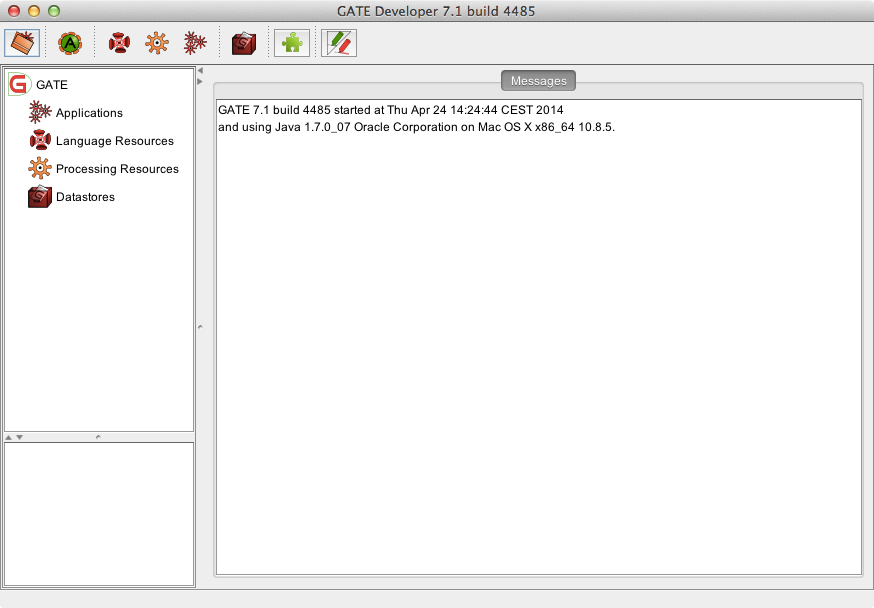
\includegraphics[scale=0.4]{POS2_Gate_nic}
				\caption{Gate interface}\label{fig:POS2}
			\end{figure}
		
		\item Consider the following text: \\\\"Apple Inc. (NASDAQ:AAPL) has announced that the Worldwide Developers Conference (WWDC) will begin on June 2. But the company is unlikely to launch the iPhone 6 at the event. The latest rumours suggest that the iPhone 6 will enter production in May and reach the public in September. As rumours build up ahead of its launch, consumers will wait for the upcoming iPhone rather than buying the current models. Let’s explore some of the latest rumours targeting its features, specifications and technologies." (Figure \ref{fig:POS1})
		
			\begin{figure}\centering
				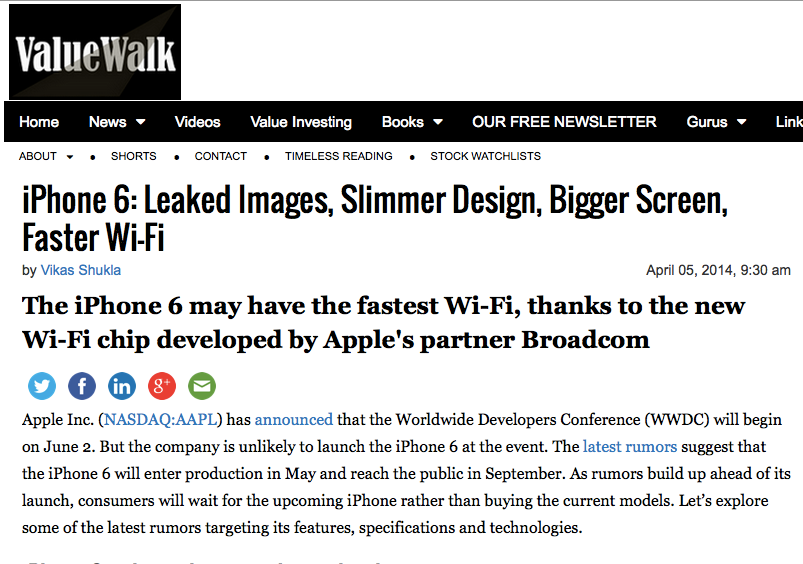
\includegraphics[scale=0.45]{POS1}
				\caption{Web page that contains the text to analyze}\label{fig:POS1}
			\end{figure}
		
		\item In "Processing Resources" add the following elements: Document reset, Tokeniser, sentence splitter, POS tagger and JAPE transducer (Don't forget to look for the "pattern.jape" file). (Figure \ref{fig:POS3}, \ref{fig:POS4})
		
			\begin{figure}\centering
				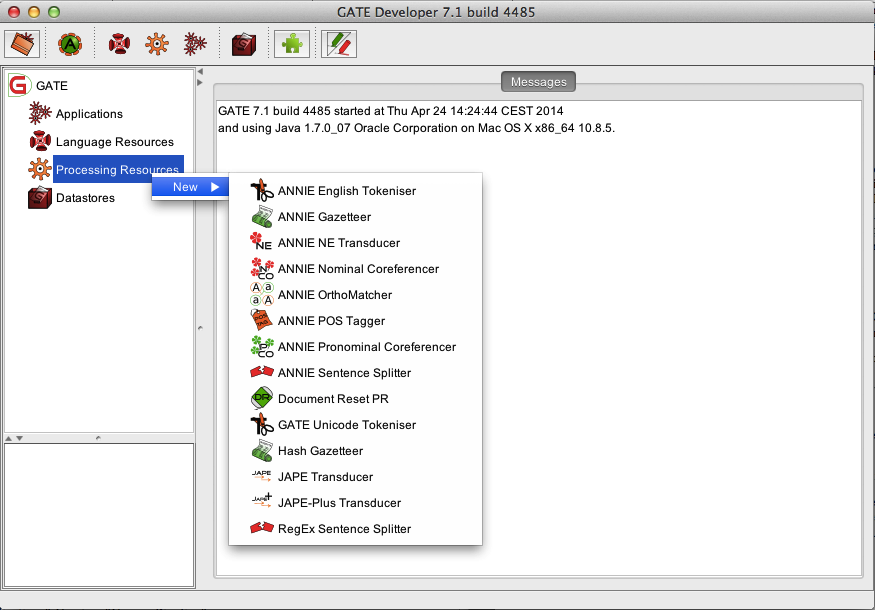
\includegraphics[scale=0.4]{POS3_Gate_processingResources}
				\caption{Processing resources available}\label{fig:POS3}
			\end{figure}

			\begin{figure}\centering
				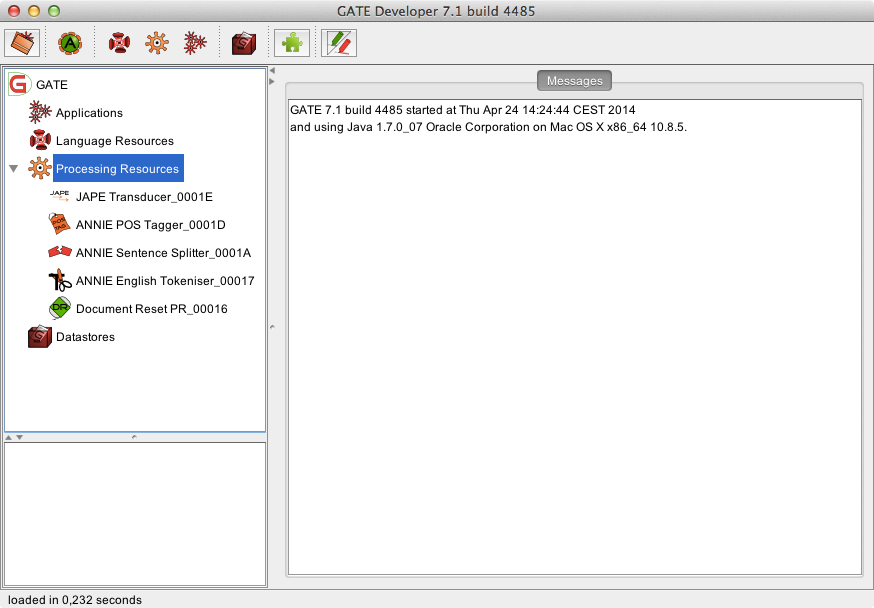
\includegraphics[scale=0.4]{POS4_Gate_ProcessingResources_2}
				\caption{Processing resources needed}\label{fig:POS4}
			\end{figure}
		
		\item In "Languages Resources" Create a "Corpus". (Figure \ref{fig:POS5})
		
			\begin{figure}\centering
				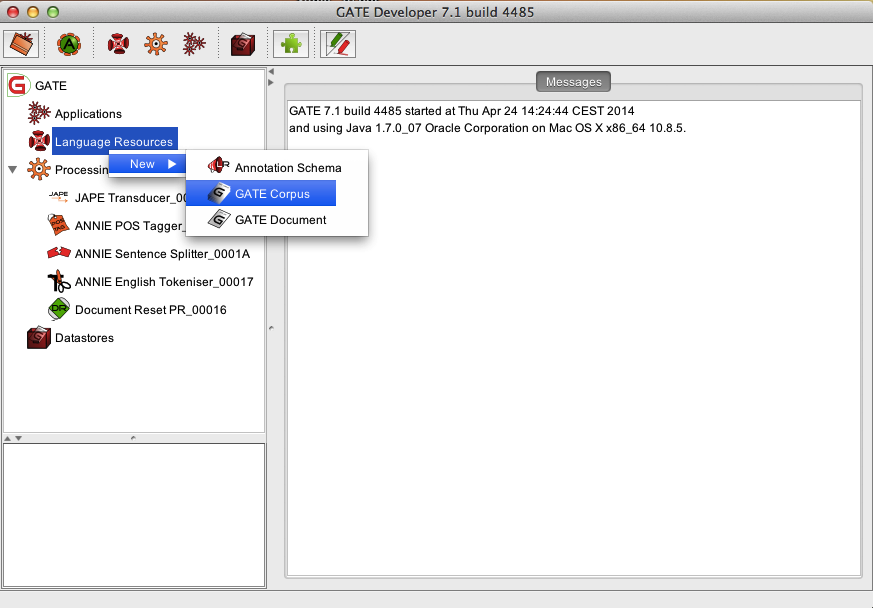
\includegraphics[scale=0.4]{POS5_Gate_LanguateResources_1}
				\caption{Language resources, Corpus \& Document}\label{fig:POS5}
			\end{figure}
		
		\item In "Languages Resources" Create a "Document". (Figure \ref{fig:POS6})
		\item Open the "Document" and paste the text that we are considering. (Figure \ref{fig:POS6})
		
			\begin{figure}\centering
				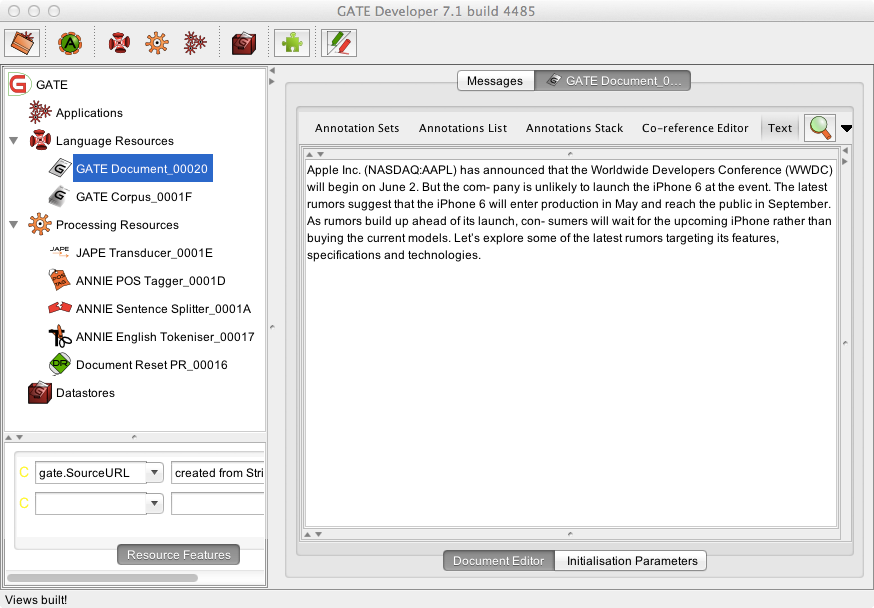
\includegraphics[scale=0.4]{POS6_Gate_LanguateResources_2}
				\caption{Language resources, Text processing}\label{fig:POS6}
			\end{figure}
		
		\item Open the "Corpus" and drag and drop the "Document" to the corpus working area. (Figure \ref{fig:POS7})
		
			\begin{figure}\centering
				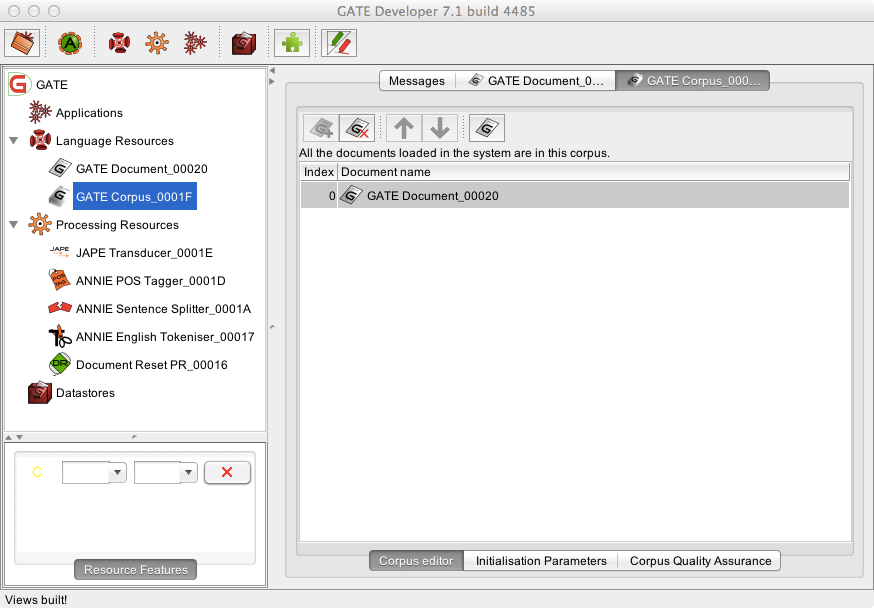
\includegraphics[scale=0.4]{POS7_Gate_LanguateResources_3}
				\caption{Language resources, Document drag \& drop to Corpus area}\label{fig:POS7}
			\end{figure}
		
		\item In "Applications" Create a "Corpus Pipeline" (Figure \ref{fig:POS8})
		
			\begin{figure}\centering
				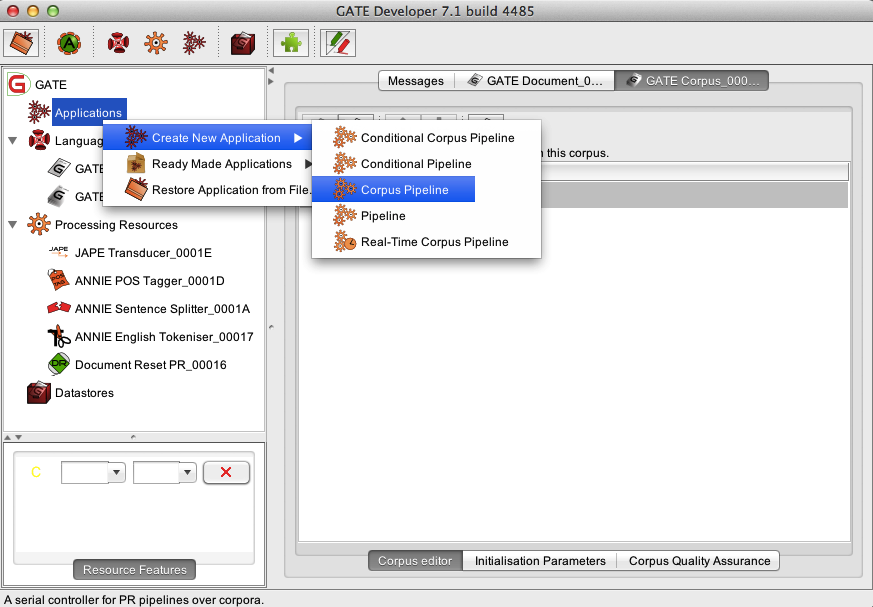
\includegraphics[scale=0.4]{POS8_Gate_Applications_1}
				\caption{Corpus creation}\label{fig:POS8}
			\end{figure}
		
		\item Open the "Corpus Pipeline", select the created "Corpus" and add the processing resources in the following order: Document reset, Tokeniser, sentence splitter, POS tagger and JAPE transducer. (Figure \ref{fig:POS9})
		
			\begin{figure}\centering
				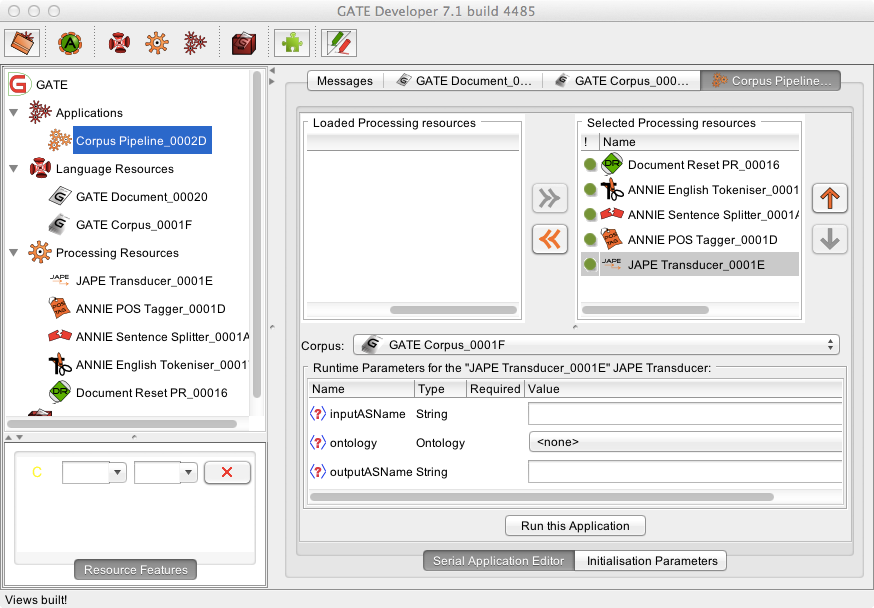
\includegraphics[scale=0.4]{POS9_Gate_Applications_2}
				\caption{Corpus setup}\label{fig:POS9}
			\end{figure}
		
		\item Press the "Run this application" button.
		\item Go back to the "Document" and press the buttons: "Annotation Sets" and "Annotation List". (Figure \ref{fig:POS10})
		
			\begin{figure}\centering
				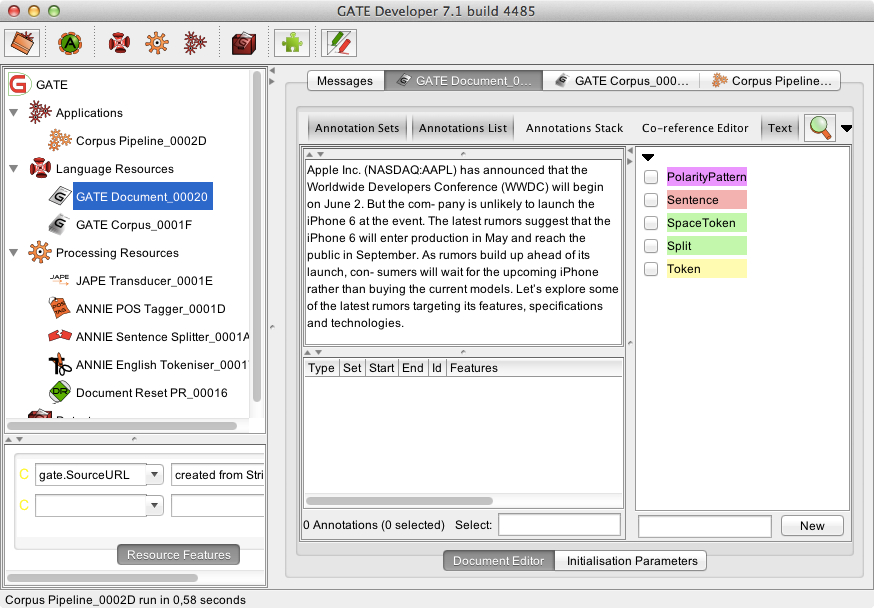
\includegraphics[scale=0.4]{POS10_Gate_Applications_3}
				\caption{Processed Document 1}\label{fig:POS10}
			\end{figure}
		
		\item After completing the previous step Click on the right: "Polarity Pattern" (Figure \ref{fig:POS10})
		\item We will see in the "Document" text marked as follows: \\\\
		Apple Inc. (NASDAQ:AAPL) has announced that the Worldwide Developers Conference (WWDC) will begin on June 2. But the company is unlikely to launch the iPhone 6 at the event. The latest rumours suggest that the iPhone 6 will enter production in May and reach the public in September. As rumours build up ahead of its launch, consumers will wait for the \textbf{\emph{upcoming iPhone}} rather than buying the \textbf{\emph{current models}}. Let’s explore some of the latest rumours targeting its features, specifications and technologies.
		\item By the time we will be running the algorithm, this two phrases were found and its neighbours words will be considered in order to calculate the polarity of the paragraph/document. (Figure \ref{fig:POS11})
		
			\begin{figure}\centering
				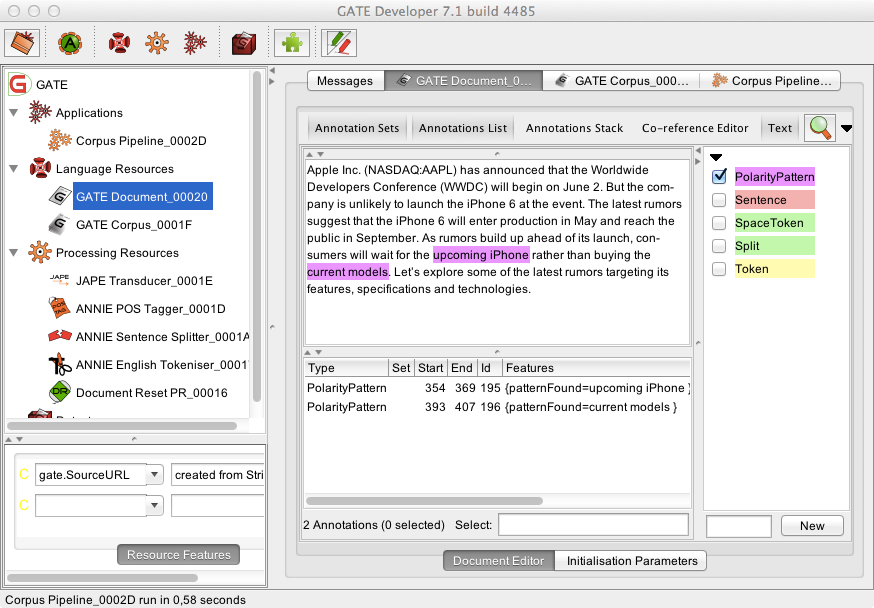
\includegraphics[scale=0.4]{POS11_Gate_Applications_4}
				\caption{Processed Document 2}\label{fig:POS11}
			\end{figure}
		
		\item This two phrases were selected according to the conditions stablished in the table \ref{tab:twoWordPhrases}. \emph{Upcoming} is adjective and \emph{iphone} is noun, and \emph{current} is adjective and \emph{models} is a noun.
	\end{itemize}
	
We already define how we will extract from the text of the article the required part-of-speech, now we will make a reference to the \emph{Pointwise mutual information} which we defined already in the section: \ref{PMI} and according to the obtained data we came to an observation; Usually authors define that reviews or texts with \emph{$PMI > $0} will be classified as \emph{positive} and \emph{$PMI \leq $0} will be classified as \emph{negative}. In this work, according to the meticulous reading of several articles (examples are shown in table: \ref{tab:FalsePositives}); when they have \emph{$0 \leq $PMI \leq $1}, the polarity of this articles even if according to some authors mathematically it is positive, in the majority of the analysed articles, their orientation is quite debatable. And in the case of finance news articles we will consider that an article should be positive enough to be consider as positive as shown in the equations \ref{eq:ourRange1} and \ref{eq:ourRange2}. With this assumption we will avoid to classify as positive anything that could be debatable, and in finances if something is debatable it \emph{should be} negative.

\begin{equation} \label{eq:ourRange1}
	-\infty \leq \operatorname{pmi}(x;y) \leq +1
\end{equation}

\begin{equation} \label{eq:ourRange2}
	+1 < \operatorname{pmi}(x;y) \leq +\infty
\end{equation}


\begin{table}\centering
	\caption{False Positives}\label{tab:FalsePositives}
   	\begin{tabular}{ | p{1.1cm\textwidth} | p{8cm\textwidth} | p{1.5cm\textwidth} | p{1.5cm\textwidth} |}
   	\hline
   	\textbf{Firma}  & \textbf{Title} & \textbf{Date} & \textbf{Score}  \\ \hline

AAPL&Samsung Electronics Co Ltd Wins Bid To Sell Nexus In Apple Inc Court Battle-Reuters&07/07/12&0.584482 \\ \hline
AAPL&Apple Inc Claims \$2.5 Billion Damages In Samsung Electronics Co Ltd Patent Case-Reuters&24/07/12&0.169725 \\ \hline
AAPL&Losers on major news: Microsoft (NASDAQ:MSFT), Citigroup (NYSE:C), Apple (NASDAQ:AAPL), Google (NASDAQ:GOOG)&28/03/14&0.405027 \\ \hline
AXP&US in talks with France on Holocaust compensation&10/04/14&0.655722 \\ \hline
BA&The Boeing Company (BA): Cash Generation May Disappoint Near-Term&13/03/14&0.777058 \\ \hline
BA&Mad Money Recommends Boeing: So Is It Time To Sell?&17/03/14&0.60467 \\ \hline
BA&"UPDATE: Malaysia Airlines MH370: 122 Objects Found In Southern Indian Ocean \& Legal Action Initiated Against Boeing And Malaysia Airlines"&26/03/14&0.705982 \\ \hline
BA&Boeing to Cut 300 Jobs in Australia as Manufacturing Weakens (1)&02/04/14&0.589379 \\ \hline
CSCO&Cisco Should Be Upgraded, Not Downgraded&19/03/14&0.870265 \\ \hline
CSCO&Cisco: Too Little, Too Late?&25/03/14&0.203206 \\ \hline
GE&GM Workers Who Built Defective Cars Fret About Recall&09/01/14&0.309883 \\ \hline
GS&Not a Good Day for Wall Street&08/04/14&0.0616087 \\ \hline
INTC&Is Intel In The Danger Zone?&20/02/14&0.646839 \\ \hline
INTC&Intel: The Worst-Case Scenario&27/02/14&0.368407 \\ \hline
INTC&Even More Bad Luck For Intel?&17/03/14&0.551018 \\ \hline
INTC&Microsoft Office For iPad Is Toxic To Intel&23/03/14&0.326464 \\ \hline
KO&Soda sales rapidly decline across the United States&31/03/14&0.430099 \\ \hline
KO&Soda sales in US drop steadily&03/04/14&0.981124 \\ \hline
MCD&McDonald's COO to retire&20/03/14&0.996407 \\ \hline
MCD&McDonald's Closes Crimean Locations&04/04/14&0.160516 \\ \hline
MCD&McDonald's Pulls Out of Crimea Due to Russian Annexation&05/04/14&0.633011 \\ \hline
    \end{tabular}
\end{table}

\subsubsection{Semantic orientation - SO}\label{SO}

According to Liu \cite%[p. 474]
{L2011},  \emph{semantic orientation} of a phrase is computed based on its association with the positive reference word “excellent” and its association with the negative reference word “poor”:

\begin{equation} \label{eq:SO1}
	SO(phrase) = PMI(phrase, "excellent") - PMI(phrase, "poor")
\end{equation}	

The probabilities are calculated by issuing queries to a search engine and collecting the number of hits. For each search query, a search engine usually gives the number of relevant documents to the query, which is the number of hits. Thus, by searching the two terms together and separately, we can estimate the probabilities in Equation \ref{eq:PMI1}. Turney, the author of \cite{T2002}, used the AltaVista search engine because it has a NEAR operator, which constrains the search to documents that contain the words within ten words of one another in either order. Let hits(query) be the number of hits returned. Equation \ref{eq:SO1} can be rewritten as:

\begin{equation} \label{eq:SO2}
\operatorname{SO}(phrase) = \log_{2}\frac{hits(phrase \operatorname{NEAR} "excelent") * hits("poor")}{hits(phrase \operatorname{NEAR} "poor") * hits("excelent")}
\end{equation}

To avoid division by zero, 0.01 is added to the hits. Let \emph{h} be the \emph{hits} and \emph{p} the \emph{phrase}.

\begin{equation} \label{eq:SO3}
\operatorname{SO}(p) = \log_{2}\frac{[ h(p \operatorname{NEAR} "excelent") + 0.01]* [ h("poor")+0.01]}{[ h(p \operatorname{NEAR} "poor") + 0.01] *[ h("excelent")+0.01]}
\end{equation}

For our purposes, we will calculate the \emph{semantic orientation} of a phrase similarly as Liu \cite{L2011}, with some modifications to adapt the algorithm to our particular needs, this is described in pseudocode in the algorithm \ref{semanticOrientationAlgorithm}. Basically, we have to load the positive and negative "bag of words"; then, according to the phrase, we will use the operator "NEAR" to search the 10 left and rightmost words. After we applied the operator "NEAR", we will search each word in the string, and we will look for \emph{positive} or \emph{negative} words, and we will account this numbers; so we can rewrite the equation \ref{eq:SO2} as:

\begin{equation} \label{eq:SO4}
\operatorname{SO}(phrase) = \log_{2}\frac{positive\_words\_phrase * negative\_words\_article}{negative\_words\_phrase * positive\_words\_article}
\end{equation}

And the equation \ref{eq:SO3} can be rewritten as: (To avoid division by zero)

\begin{equation} \label{eq:SO5}
\operatorname{SO}(phrase) = \log_{2}\frac{(positive\_words\_phrase+0.01) * (negative\_words\_article+0.01)}{(negative\_words\_phrase+0.01) * (positive\_words\_article+0.01)}
\end{equation}

The equation \ref{eq:SO5} is the one that will be used in the implementation of the \emph{semantic orientation} in the framework, and as a result we will obtain a real number.

As we know, every article will have \emph{N} phrases that will fulfill the requirements of the table \ref{tab:twoWordPhrases}, so we will have one score for the semantic orientation for each of the \emph{N} phrases; to get the score of the document we will compute the average of all the scores of each \emph{semantic orientation} from each phrase, as it will be defined in the equation: \ref{eq:avgSO}

\begin{equation} \label{eq:avgSO}
\overline{SO} = \frac {1}{N} \sum_{n=1}^{N} SO(phrase_n) \\	
\end{equation}


\subsubsection{The unsupervised learning algorithm}\label{theUnsuervisedAlgorithm}

Now, that we that we have introduced the theory that is behind \emph{the unsupervised learning algorithm} (Part of speech (section: \ref{partOfSpeech}), Pointwise mutual information (section: \ref{PMI}) and Semantic Orientation (section: \ref{SO})), we will present the algorithm used in our work, this is shown as pseudo code in the algorithm \ref{unsupervisedAlgorithm}. The base algorithm will be according to Liu \cite%[p. 473,474]
{L2011}.

The algorithm has 3 steps:
	\begin{itemize}
		\item \emph{Phase 1:} Extract phrases containing adjectives or adverbs as adjectives and adverbs are good indicators of opinions. The algorithm extracts two consecutive words, where one member of the pair is an adjective or adverb, and the other is a context word. Two consecutive words are extracted if their POS tags conform to any of the patterns in table \ref{tab:twoWordPhrases}. For example, the pattern in the second line means that two consecutive words are extracted if the first word is an adverb and the second word is an adjective.
		\item \emph{Phase 2:} Estimate the semantic orientation of the extracted phases using the \emph{PMI - Pointwise Mutual Information} (\ref{PMI}), using the equation: \ref{eq:SO5}. 
		\item \emph{Phase 3:} Given some text; in our case an \emph{Article}, the algorithm computes the average semantic orientation (algorithm \ref{semanticOrientationAlgorithm}, equation: \ref{eq:avgSO}) of all phrases in the \emph{Article} and classify the review according to the equations  \ref{eq:ourRange1} and \ref{eq:ourRange2}.
	\end{itemize}

\begin{algorithm}
\caption{Unsupervised classification algorithm}\label{unsupervisedAlgorithm}
\begin{algorithmic}[1]
\STATE \text{\emph{Input: article; Output: Average Semantic Orientation.}}
\STATE \text{Load positive "Bag of words";}
\STATE \text{Load negative "Bag of words";}
\STATE \text{Count \emph{positive\_words\_in\_article;}}

\STATE \text{Count} \emph{negative\_words\_in\_article;}
\STATE \text{Phase 1:}
	\STATE \text{Extract} \emph{phrases} containing indicators of \emph{opinions}
\STATE \text{Phase 2:}
	\FOR {\text{each} \emph{phrase} \text{found}}
		\STATE \text{Calculate \emph{semantic orientation} of the \emph{phrase};}
	\ENDFOR
\STATE \text{Phase 3:}
	\STATE \text{Compute the average \emph{semantic orientation} of all \emph{phrases};}
\STATE \text{return \emph{average semantic orientation};}
\end{algorithmic}
\end{algorithm}

\begin{algorithm}
\caption{Semantic orientation algorithm}\label{semanticOrientationAlgorithm}
\begin{algorithmic}[1]
\STATE \text{\emph{Input: Article, phrase, positive\_words, negative\_words; Output: Phrase SO.}}
\STATE \text{wordArray := NEAR(Article text, phrase);}
\FOR {\text{each} \emph{word} \text{in WordArray}}
	\STATE \text{\emph{search} word in \emph{positive} "Bag of words"and account it;}
	\IF{positive\_word\_found}
	\STATE \text{hits\_positive++}
	\ENDIF
	\STATE \text{\emph{search} word in \emph{negative} "Bag of words" and account it;}
	\IF{negative\_word\_found}
	\STATE \text{hits\_negative++}
	\ENDIF
\ENDFOR
\RETURN \text{\emph{PMI}}
\end{algorithmic}
\end{algorithm}

Now we have the theoretical background needed in order to start implementing the framework. In the next chapter, we will define all the technical details that we had to solve in order to deliver the framework.
